\chapter{Описание стенда и подготовка}
\label{ch:stand}

\section{Конфигурация виртуального стенда}

Виртуальная машина \texttt{gateway}~— Ubuntu~20.04.5~LTS (VirtualBox),
два сетевых адаптера:
\begin{itemize}
  \item \textbf{Адаптер~1} (\texttt{enp0s3}) — тип \textit{NAT}:
        IP \texttt{10.0.2.15/24}, шлюз \texttt{10.0.2.2};
  \item \textbf{Адаптер~2} (\texttt{enp0s8}) — тип \textit{Internal Network}:
        IP \texttt{192.168.\cfgLabStudentN.1/24}.
\end{itemize}

К началу лаб.~работы~\cfgLabNumber{} на \texttt{gateway} уже функционируют:
DNS-сервер BIND9, DHCP-сервер \texttt{isc-dhcp-server},
маршрутизация с iptables MASQUERADE.

Виртуальная машина \texttt{mail}~— Ubuntu~22.04~LTS~Server:
\begin{itemize}
  \item \textbf{Адаптер~1} (\texttt{enp0s3}) — тип \textit{Internal Network},
        статический IP \texttt{192.168.\cfgLabStudentN.5/24}.
\end{itemize}

% — Скриншот: настройки ВМ mail в VirtualBox (вкладка Сеть) —
\begin{figure}[h]
  \centering
  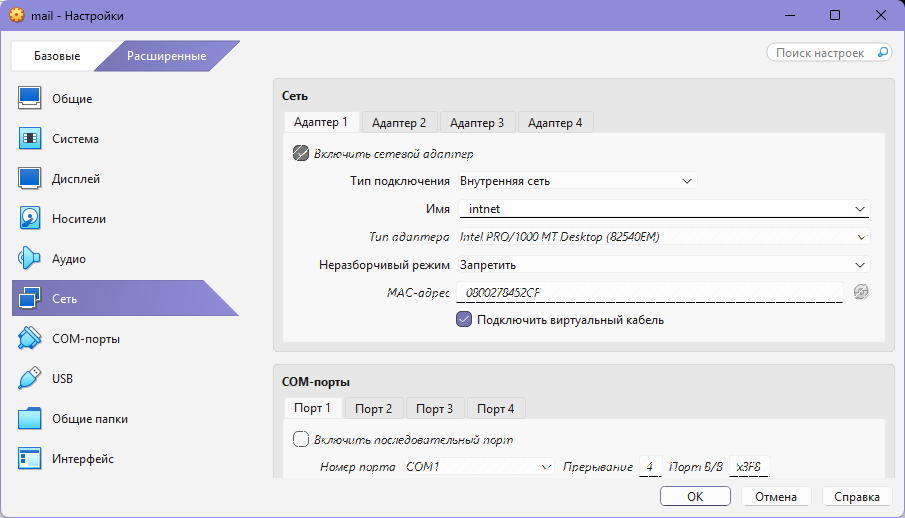
\includegraphics[width=0.85\textwidth]{img/01_vbox_mail_network}
  \caption{Настройки сети ВМ \texttt{mail} в VirtualBox}
  \label{fig:vbox_mail}
\end{figure}

\section{Настройка сети на mail}

После установки Ubuntu~22.04 настраиваем статический IP с помощью netplan.

\begin{lstlisting}
nano /etc/netplan/01-netcfg.yaml
\end{lstlisting}

\begin{lstlisting}
network:
  version: 2
  renderer: networkd
  ethernets:
    enp0s3:
      dhcp4: no
      addresses:
        - 192.168.N.5/24
      gateway4: 192.168.N.1
      nameservers:
        addresses: [192.168.N.1]
\end{lstlisting}

\begin{lstlisting}
netplan apply
ip a
\end{lstlisting}

% — Скриншот: вывод ip a на mail (192.168.N.5 на enp0s3) —
\begin{figure}[h]
  \centering
  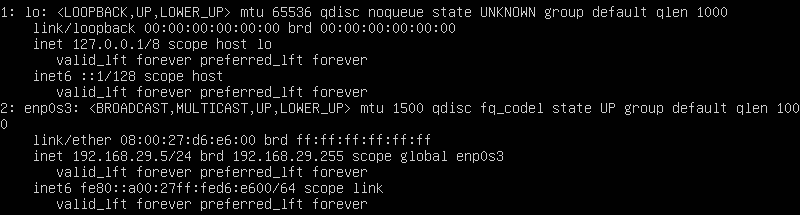
\includegraphics[width=0.85\textwidth]{img/02_mail_ip_a}
  \caption{Вывод \texttt{ip a} на ВМ \texttt{mail}: адрес 192.168.\cfgLabStudentN.5}
  \label{fig:mail_ip}
\end{figure}

\section{Проверка связи и DNS}

Проверяем доступность шлюза, интернета и разрешение имён:

\begin{lstlisting}
ping -c 4 192.168.N.1
nslookup gateway.\cfgDomain
\end{lstlisting}

% — Скриншот: ping до gateway и nslookup —
\begin{figure}[h]
  \centering
  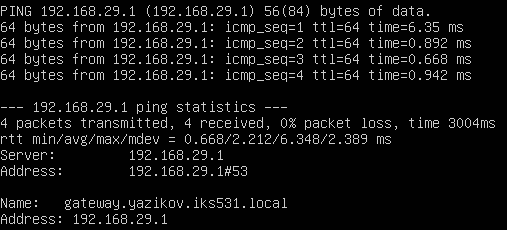
\includegraphics[width=0.85\textwidth]{img/03_mail_ping_nslookup}
  \caption{Проверка сетевой связи и DNS с ВМ \texttt{mail}}
  \label{fig:mail_ping}
\end{figure}

\section{Настройка имени хоста}

iRedMail требует полностью определённого FQDN-имени хоста.
Задаём его командой \texttt{hostnamectl}, затем прописываем в
\texttt{/etc/hosts}:

\begin{lstlisting}
hostnamectl set-hostname mail.\cfgDomain
nano /etc/hosts
\end{lstlisting}

Содержимое \texttt{/etc/hosts}:
\begin{lstlisting}
127.0.0.1  mail.\cfgDomain  mail  localhost
192.168.N.5  mail.\cfgDomain  mail
\end{lstlisting}

% — Скриншот: nano /etc/hosts с прописанным FQDN —
\begin{figure}[h]
  \centering
  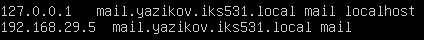
\includegraphics[width=0.85\textwidth]{img/04_mail_etc_hosts}
  \caption{Файл \texttt{/etc/hosts} с FQDN-именем \texttt{mail.\cfgDomain}}
  \label{fig:mail_hosts}
\end{figure}

\section{Добавление записи в DNS на gateway}

На ВМ \texttt{gateway} добавляем A-запись \texttt{mail} в файл прямой зоны
и перезапускаем BIND9:

\begin{lstlisting}
nano /var/lib/bind/forward.db
\end{lstlisting}

Добавить строку:
\begin{lstlisting}
mail  IN A  192.168.N.5
\end{lstlisting}

\begin{lstlisting}
systemctl restart bind9
nslookup mail.\cfgDomain
\end{lstlisting}

% — Скриншот: nslookup mail.\cfgDomain (успешно) —
\begin{figure}[h]
  \centering
  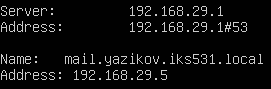
\includegraphics[width=0.85\textwidth]{img/05_dns_mail_record}
  \caption{Проверка DNS-записи \texttt{mail.\cfgDomain}}
  \label{fig:dns_mail}
\end{figure}

\endinput
